\documentclass[fleqn]{MJD}

\usepackage{cancel}
\usepackage{cleveref}
\usepackage{titlesec}
\usepackage{hyperref}
%\colorsections
%\bluelinks
\newcommand{\problem}[1]{\chapter{Problem #1}}
\newcommand{\subproblem}[2]{\section{(#1)~ #2}}
\newcommand{\subsubproblem}[2]{\subsection{ #1)~ #2}}
\newcommand{\U}{\cup}
\renewcommand{\S}{\mathcal{S}}
\renewcommand{\s}{\subset}
\renewcommand{\equiv}{\Leftrightarrow}
\newcommand{\0}{\emptyset}
\newcommand{\imp}{\Rightarrow}
\newcommand{\Usum}{\bigcup\limits_{i=1}^\infty}
\newcommand{\intsum}{\bigcup\limits_{i=1}^\infty}
\newcommand{\infsum}{\sum\limits_{i=1}^\infty}
\newcommand{\sets}{\{A_1, A_2 \dots\} }
\newcommand{\nsets}{\{A_1, \dots, A_n \} }

\titleformat{\chapter}[display]
  {\normalfont\bfseries}{}{0pt}{\LARGE}
  
\graphicspath{ {../Code/} }

%%%%%%%%%%%%%%%%%%%%%%%%%%%%%%%%%%%%
\begin{document}

\titleAT[CS 224N: Assignment 1]{Ryan McMahon}
\large

\begingroup
\let\clearpage\relax
\tableofcontents
\endgroup
\newpage

%-------------------------------------
\problem{1: Softmax (10 pts)}
%-------------------------------------

%----------------------
\subproblem{a}{Softmax Invariance to Constant (5 pts)}
\textit{Prove that softmax is invariant to constant offsets in the input, that is, for any input vector $x$ and any constant $c$, softmax($x$) = softmax($x + c$), where $x + c$ means adding the constant $c$ to every dimension of $x$. Remember that} 
\begin{equation}
	softmax(x)_{i} = \frac{e^{x_{i}}}{\sum_{j} e^{x_{j}}}
\end{equation}


\noindent\textbf{Answer:} \\

\noindent We can show that softmax($x$) = softmax($x+c$) by factoring out $c$ and canceling:

\begin{align}
	softmax(x + c)_{i} &= \frac{e^{x_{i} + c}}{\sum_{j} e^{x_{j} + c}} %
	 					= \frac{e^{x_{i}} \times e^{c}}{e^{c} \times \sum_{j} e^{x_{j}}} \nonumber \\
	%
					   &= \frac{e^{x_{i}} \times \cancel{e^{c}}}{\cancel{e^{c}} \times \sum_{j} e^{x_{j}}} %
					    = softmax(x)_{i} \nonumber
\end{align}

\vskip5em

%----------------------
\subproblem{b}{Softmax Coding (5 pts)}
\textit{Given an input matrix of $N$ rows and $D$ columns, compute the softmax prediction for each
row using the optimization in part (a). Write your implementation in} \verb|q1_softmax.py|. \textit{You may test
by executing} \verb|python q1_softmax.py|. \\

\noindent\textit{Note: The provided tests are not exhaustive. Later parts of the assignment will reference this code so it is important to have a correct implementation. Your implementation should also be efficient and vectorized whenever possible (i.e., use numpy matrix operations rather than for loops). A non-vectorized implementation will not receive full credit!} \\

\noindent \textbf{Answer:} \\

\noindent See code: $\sim$\verb|/code/q1_softmax.py|.



\newpage
%-------------------------------------
\problem{2: Neural Network Basics (30 pts)}
%-------------------------------------


%----------------------
\subproblem{a}{Sigmoid Gradient (3 pts)}

\textit{Derive the gradients of the sigmoid function and show that it can be rewritten as a function of the function value (i.e., in some expression where only σ(x), but not x, is present). Assume that the input x is a scalar for this question. Recall, the sigmoid function is}

\begin{equation}
	\sigma(x) = \frac{1}{1 + e^{-x}}
\end{equation}


\noindent \textbf{Answer:}

\begin{align}
	\sigma(x) &= \frac{1}{1 + e^{-x}} \nonumber \\
	%
			  &= \frac{e^{x}}{1 + e^{x}} \nonumber \\
	%
	\frac{\partial}{\partial x} \sigma(x) &= \frac{e^{x} \times (1 + e^{x}) - (e^{x} \times e^{x})}{(1 + e^{x})^{2}} \nonumber \\
	%
			  &= \frac{e^{x} + \cancel{(e^{x} \times e^{x})} - \cancel{(e^{x} \times e^{x})}}{(1 + e^{x})^{2}} \nonumber \\
	%
			  &= \frac{e^{x}}{(1 + e^{x})^{2}}  = \sigma(x) \times (1 - \sigma(x)) \nonumber 
\end{align}

\vskip2em
\noindent Because $1 - \sigma(x) = \sigma(-x)$ we can show that:

\begin{align}
	\frac{\partial}{\partial x} \sigma(x) &= \frac{e^{x}}{(1 + e^{x})^{2}} \nonumber \\
	%
			  &= \sigma(x) \times \sigma(-x) \nonumber \\
	%
			  &= \frac{e^{x}}{1 + e^{x}} \times \frac{1}{1 + e^{+x}} \nonumber \\
	%
			  &= \frac{e^{x}}{(1 + e^{x})^{2}} \nonumber
\end{align}



%----------------------
\newpage
\subproblem{b}{Softmax Gradient w/ Cross Entropy Loss (3 pts)}
\label{prob:2b}

\textit{Derive the gradient with regard to the inputs of a softmax function when cross entropy loss is used for evaluation, i.e., find the gradients with respect to the softmax input vector $\bm{\theta}$, when the prediction is made by $\hat{\mathbf{y}} = softmax(\bm{\theta})$. Remember the cross entropy function is}

\begin{equation}
	CE(\mathbf{y},\hat{\mathbf{y}}) = - \sum_{i} y_{i} \times log(\hat{y_{i}})
\end{equation}

\noindent \textit{where $\mathbf{y}$ is the one-hot label vector, and $\hat{\mathbf{y}}$ is the predicted probability vector for all classes. (Hint: you might want to consider the fact many elements of $\mathbf{y}$ are zeros, and assume that only the $k-th$ dimension
of $\mathbf{y}$ is one.)} \\

\noindent \textbf{Answer:} \\

\noindent Let $S$ represent the softmax function:

\begin{align}
	f_{i} &= e^{\theta_{i}} \nonumber \\
	%
	g_{i} &= \sum_{k=1}^{K} e^{\theta_{k}} \nonumber \\
	%
	S_{i} &= \frac{f_{i}}{g_{i}} \nonumber \\
	%
	\frac{\partial S_{i}}{\partial \theta_{j}} &= \frac{f'_{i} g_{i} - g'_{i} f_{i}}{g_{i}^{2}} \nonumber
\end{align}

\vskip2em
%
\noindent So if $i = j$:
\begin{align}
	f'_{i} &= f_{i}; \hspace*{5pt} g'_{i} = e^{\theta_{j}} \nonumber \\
	%
	\frac{\partial S_{i}}{\partial \theta_{j}} &= \frac{e^{\theta_{i}} \sum_{k} e^{\theta_{k}} - e^{\theta_{j}} e^{\theta_{i}} }{ (\sum_{k} e^{\theta_{k}})^{2} } \nonumber \\
	%
		   &= \frac{e^{\theta_{i}}}{\sum_{k} e^{\theta_{k}}} \times \frac{\sum_{k} e^{\theta_{k}} - e^{\theta_{j}}}{\sum_{k} e^{\theta_{k}}} \nonumber \\
	%
		   &= S_{i} \times (1 - S_{i}) \nonumber
\end{align}

\vskip2em
%
\noindent And if $i \ne j$:
\begin{align}
	\frac{\partial S_{i}}{\partial \theta_{j}} %
		&= \frac{0 - e^{\theta_{j}} e^{\theta_{i}}}{(\sum_{k} e^{\theta_{k}})^{2}} \nonumber \\
	%
		&= - \frac{e^{\theta_{j}}}{\sum_{k} e^{\theta_{k}}} \times \frac{e^{\theta_{i}}}{\sum_{k} e^{\theta_{k}}} \nonumber \\
	%
		&= -S_{j} \times S_{i} \nonumber
\end{align}

\newpage

\noindent We can now use these when operating on our loss function (let $L$ represent the cross entropy function):
\begin{align}
	\frac{\partial L}{\partial \theta_{i}} % 
		&= - \sum_{k} y_{k} \frac{\partial log S_{k}}{\partial \theta_{i}}	\nonumber \\
	%
		&= - \sum_{k} y_{k} \frac{1}{S_{k}} \frac{\partial S_{k}}{\partial \theta_{i}} \nonumber \\
	%
		&= - y_{i} (1 - S_{i}) - \sum_{k \ne i} y_{k} \frac{1}{S_{k}} (-S_{k} \times S_{i}) \nonumber \\
	% 
		&= - y_{i} (1 - S_{i}) + \sum_{k \ne i} y_{k} S_{i} \nonumber \\
	%
		&= - y_{i} + y_{i} S_{i} + \sum_{k \ne i} y_{k} S_{i} \nonumber \\
	%
		&= S_{i}(\sum_{k} y_{k}) - y_{i} \nonumber
\end{align}

\vskip2em

\noindent And because we know that $\sum_{k} y_{k} = 1$:
\begin{align}
	\frac{\partial L}{\partial \theta_{i}} % 
			&= S_{i} - y_{i} \nonumber
\end{align} 



%----------------------
\newpage
\subproblem{c}{One Hidden Layer Gradient (6 pts)}

\textit{Derive the gradients with respect to the inputs $\bm{x}$ to a one-hidden-layer neural network (that is, find $\frac{\partial J}{\partial \bm{x}}$ where $J = CE(\mathbf{y}, \hat{\mathbf{y}})$ is the cost function for the neural network). The neural network employs sigmoid activation function for the hidden layer, and softmax for the output layer. Assume the one-hot label vector is $\mathbf{y}$, and cross entropy cost is used. (Feel free to use $\sigma'(x)$ as the shorthand for sigmoid gradient, and feel free to define any variables whenever you see fit.)} \\

\noindent \textit{Recall that forward propoagation is as follows}
\begin{align}
	\mathbf{h} &= sigmoid(\bm{xW}_{1} + \bm{b}_{1})	& \hat{\bm{y}} = softmax(\bm{hW}_{2} + \bm{b}_{2}) \nonumber
\end{align}

\vskip2em

\noindent \textbf{Answer:} \\

\noindent Let $f_{2} = \bm{xW}_{1} + \bm{b}_{1}$ and $f_{3} = \bm{hW}_{2} + \bm{b}_{2}$;

\begin{align}
	\frac{\partial J}{\partial f_{3}} %
		&= \bm{\delta}_{3} = \hat{\bm{y}} - \bm{y} \nonumber \\
	%
	\frac{\partial J}{\partial \bm{h}} %
		&= \bm{\delta}_{2} = \bm{\delta}_{3}\bm{W}_{2}^{T} \nonumber \\
	%
	\frac{\partial J}{\partial f_{2}} %
			&= \bm{\delta}_{1} = \bm{\delta}_{2} \circ \sigma'(f_{2}) \nonumber \\
	%
	\frac{\partial J}{\partial \bm{x}} %
		&= \bm{\delta}_{1} \frac{\partial f_{2}}{\partial \bm{x}} \nonumber \\
	%
		&= \bm{\delta}_{1}  \bm{W}_{1}^{T} \nonumber
\end{align}

\vskip5em

%----------------------
\subproblem{d}{No. Parameters (2 pts)}

\textit{How many parameters are there in this neural network} [from (\textbf{c}) above], \textit{assuming the input is $D_{x}-$dimensional, the output is $D_{y}-$dimensional, and there are $H$ hidden units?} \\

\noindent \textbf{Answer:} \\

\begin{align}
	n_{W_{1}} &= D_{x} \times H \nonumber \\
	%
	n_{b_{1}} &= H \nonumber \\
	%
	n_{W_{2}} &= H \times D_{y} \nonumber \\
	%
	n_{b_{2}} &= D_{y} \nonumber \\
	%
	N &= (D_{x} \times H) + H + (H \times D_{y}) + D_{y} \nonumber
\end{align}



%----------------------
\newpage
\subproblem{e}{Sigmoid Activation Code (4 pts)}

\textit{Fill in the implementation for the sigmoid activation function and its gradient in} \verb|q2_sigmoid.py|. \textit{Test your implementation using} \verb|python q2_sigmoid.py|. \textit{Again, thoroughly test your code as the provided tests may not be exhaustive.} \\

\noindent \textbf{Answer:} \\

\noindent See code: $\sim$\verb|/code/q2_sigmoid.py|.

\vskip5em


%----------------------
\subproblem{f}{Gradient Check Code (4 pts)}

\textit{To make debugging easier, we will now implement a gradient checker. Fill in the implementation for} \verb|gradcheck_naive| \textit{in} \verb|q2_gradcheck.py|. \textit{Test your code using} \verb|python q2_gradcheck.py|. \\

\noindent \textbf{Answer:} \\

\noindent See code: $\sim$\verb|/code/q2_gradcheck.py|.

\vskip5em


%----------------------
\subproblem{g}{Neural Net Code (8 pts)}

\textit{Now, implement the forward and backward passes for a neural network with one sigmoid hidden layer. Fill in your implementation in} \verb|q2_neural.py|. \textit{Sanity check your implementation with} \verb|python q2_neural.py|. \\

\noindent \textbf{Answer:} \\

\noindent See code: $\sim$\verb|/code/q2_neural.py|.



\newpage

%-------------------------------------
\problem{3: Word2Vec (40 pts + 2 bonus)}
%-------------------------------------

%----------------------
\subproblem{a}{Context Word Gradients (3 pts)}

\textit{Assume you are given a predicted word vector $\bm{v}_{c}$ corresponding to the center word $\bm{c}$ for skipgram, and word prediction is made with the softmax function found in word2vec models}

\begin{align}
	\hat{\bm{y}}_{o} &= p(\bm{o} \hspace*{1pt} \vert \hspace*{1pt} \bm{c}) = %
					\frac{exp(\bm{u}_{0}^{T} \bm{v}_{c})}{\sum\limits_{w=1}^{W} exp(\bm{u}_{w}^{T} \bm{v}_{c})}
\end{align}

\noindent \textit{where $\bm{w}$ denotes the w-th word and $\bm{u}_{w}$ ($w = 1,...,W$) are the ``output'' word vectors for all words in the vocabulary. Assume cross entropy cost is applied to this prediction and word $\bm{o}$ is the expected word (the $\bm{o}$-th element of the one-hot label vector is one), derive the gradients with respect to $\bm{v}_c$, } \\

Hint: It will be helpful to use notation from question 2. For instance, letting $\hat{\bm{y}}$ be the vector of softmax predictions for every word, $\bm{y}$ as the expected word vector, and the loss function

\begin{align}
	J_{softmax-CE}(\bm{o}, \bm{v}_{c}, \bm{U}) &= CE(\bm{y}, \hat{\bm{y}})
\end{align}

\noindent \textit{where $\bm{U}$ = [$\bm{u}_{1}$,$\bm{u}_{1}$,$\dots$, $\bm{u}_{W}$] is the matrix of all the output vectors. Make sure you state the orientation of your vectors and matrices.} \\


\noindent \textbf{Answer:} \\

\noindent From Problem~\ref{prob:2b} we know that $\frac{\partial J}{\partial \bm{\theta}} = (\hat{\bm{y}} - \bm{y})$. Given that, let $\bm{theta} = \bm{v}_{c}$. Then 

\begin{align}
	\frac{\partial J}{\partial \bm{\theta}} &= %
	 		\bm{U}^{T} (\hat{\bm{y}} - \bm{y}) \nonumber
\end{align}



\newpage
%----------------------
\subproblem{b}{Output Word Gradients (3 pts)}

\textit{As in the previous part, derive gradients for the “output” word vectors $\bm{u}_{w}$ 's (including $\bm{u}_{o}$).} \\

\noindent \textbf{Answer:} \\

\noindent Here we're going to do essentially the same thing, but instead transpose the error. So, from above and Problem~\ref{prob:2b}, let $\bm{\theta} = \bm{U}$


\begin{align}
	\frac{\partial J}{\partial \bm{\theta}} &= %
		 		\bm{v}_{c} (\hat{\bm{y}} - \bm{y})^{T} \nonumber
\end{align}

\vskip5em



%----------------------
\subproblem{c}{Repeat Gradients with Negative Sampling Loss (6 pts)}

\textit{Repeat part \textbf{(a)} and \textbf{(b)} assuming we are using the negative sampling loss for the predicted vector $\bm{v}_{c}$, and the expected output word is $\bm{o}$. Assume that $\bm{K}$ negative samples (words) are drawn, and they are $\bm{1},\dots ,\bm{K}$, respectively for simplicity of notation ($o \notin \{1,...,K\}$). Again, for a given word, $o$,denote its output vector as $\bm{u}_{o}$. The negative sampling loss function in this case is}

\begin{align}
	J_{neg-sample}(\bm{o}, \bm{v}_{c}, \bm{U}) &= %
		− log(\sigma(\bm{u}_{o}^{T} \bm{v}_{c})) - \sum\limits_{k=1}^{K} log(\sigma(-\bm{u}_{k}^{T} \bm{v}_{c}))
\end{align}

\noindent where $\sigma(\cdot)$ is the sigmoid function. \\

\noindent \textit{After you’ve done this, describe with one sentence why this cost function is much more efficient to compute than the softmax-CE loss (you could provide a speed-up ratio, i.e. the runtime of the softmax-CE loss divided by the runtime of the negative sampling loss).} \\


\noindent \textbf{Answer:} \\

\noindent Let $z_{j} = \bm{u}_{j}^{T} \bm{v}_{c}$:

\begin{align}
	\frac{\partial J}{\partial z_{j}} &= %
		\left\{
			\begin{array}{ll}
				 \sigma(\bm{u}_{j}^{T} \bm{v}_{c}) - 1 & \mbox{if } j = o \\ 
				 \sigma(\bm{u}_{j}^{T} \bm{v}_{c}) 	   & \mbox{if } j \in \bm{K}
			\end{array}
		\right. \nonumber 
\end{align}

\noindent Then we can separate out the partials for $\bm{u}_{j}$ and $\bm{v}_{c}$.

\begin{align}
	\frac{\partial J}{\partial \bm{u}_{o}} &= %
		\frac{\partial J}{\partial z_{j}} \times %
			\frac{ \partial z_{j} }{ \partial \bm{u}_{o} } \nonumber \\
		%
		&= (\sigma(\bm{u}_{o}^{T} \bm{v}_{c}) - 1) \bm{v}_{c} \nonumber \\
	%
	\frac{\partial J}{\partial \bm{u}_{k}} &= %
			\frac{\partial J}{\partial z_{j}} \times %
				\frac{ z_{j} }{ \partial \bm{u}_{k} } \nonumber \\
		%
		&= -(\sigma(-\bm{u}_{k}^{T} \bm{v}_{c}) - 1) \bm{v}_{c} \mbox{  for all } k \in \bm{K} \nonumber
\end{align}

\begin{align}
	\frac{\partial J}{\partial \bm{v}_{c}} &= %
		\frac{\partial J}{\partial z_{j}} \times %
			\frac{ \partial z_{j}}{ \partial \bm{v}_{c} } \nonumber \\
		%
		&= (\sigma(\bm{u}_{o}^{T} \bm{v}_{c}) -1) \bm{u}_{o} - %
			\sum\limits_{k=1}^{K} (\sigma(- \bm{u}_{k}^{T} \bm{v}_{c}) - 1) \bm{u}_{k} \nonumber
\end{align}


\noindent This is faster than the original cross entropy loss because we are no longer deriving the gradients $\forall w_{j} \in W$. Instead, we are only evaluating the gradients for $[w_{o}, w_{k},\dots,w_{K}]$. 


\vskip5em


%----------------------
\subproblem{d}{Skip-gram and CBOW Gradients (8 pts)}
\textit{Derive gradients for all of the word vectors for skip-gram and CBOW given the previous parts and given a set of context words [word$_{c−m}$ ,...,word$_{c−1}$ ,word$_{c}$ ,word$_{c+1}$ ,...,word$_{c+m}$ ], where $m$ is the context size. Denote the “input” and “output” word vectors for word $k$ as $v_{k}$ and $u_{k}$ respectively.} \\

\noindent \textit{Hint: Feel free to use $F(\bm{o}, \bm{v}_{c})$ (where $\bm{o}$ is the expected word) as a placeholder for the $J_{softmax-CE}(\bm{o},\bm{v}_{c},\dots)$ or $J_{neg-sample}(\bm{o},\bm{v}_{c},\dots)$ cost functions in this part -- you'll see that this is a useful abstraction for the coding part. That is, your solution may contain terms of the form $\frac{\partial F(\bm{o}, \bm{v}_{c})}{\partial \dots}$.} \\
%
\noindent \textit{Recall that for skip-gram, the cost for a context centered around $c$ is }
%
\begin{align}
	J_{skip-gram}(word_{c-m \dots c+m}) &= %
		\sum\limits_{-m \leq j \leq m, j \ne 0} F(\bm{w}_{c+j}, \bm{v}_{c}) 
\end{align}
\noindent \textit{where $\bm{w}_{c+j}$ refers to the word at the $j-$th index from the center.} \\

\noindent \textit{CBOW is slightly different. Instead of using $\bm{v}_{c}$ as the predicted vector, we use $\hat{\bm{v}}$ defined below. For (a simpler variant of) CBOW, we sum up the input word vectors in the context}
%
\begin{align}
	\hat{\bm{v}} &= \sum\limits_{-m \leq j \leq m, j \ne 0} \bm{v}_{c+j}
\end{align}
\noindent then the CBOW cost is
%
\begin{align}
	J_{CBOW}(word_{c-m \dots c+m}) &= F(\bm{w}_{c}, \hat{\bm{v}})
\end{align}

\noindent \textit{Note: To be consistent with the $\hat{\bm{v}}$ notation such as for the code portion, for skip-gram $\hat{\bm{v}} = \bm{v}_{c}$.} \\


\noindent \textbf{Answer:} \\

\noindent For the skip-gram model, we can show that (for a given context window) the gradients are equal to:
%
\begin{align}
	\frac{J_{skip-gram}(word_{c-m \dots c+m})}{\partial \bm{U}} &= %
		\sum\limits_{-m \leq j \leq m, j \ne 0} \frac{\partial F(\bm{w}_{c+j}, \bm{v}_{c})}{\partial \bm{U}} \nonumber \\
	%
	\frac{J_{skip-gram}(word_{c-m \dots c+m})}{\partial \bm{v}_{c}} &= %
		\sum\limits_{-m \leq j \leq m, j \ne 0} \frac{\partial F(\bm{w}_{c+j}, \bm{v}_{c})}{\partial \bm{v}_{c}} \nonumber \\
	%
	\frac{J_{skip-gram}(word_{c-m \dots c+m})}{\partial \bm{v}_{j}} &= 0, \forall j\ne c \nonumber
\end{align}


\noindent For the CBOW model, alternatively, the gradients are equal to:
%
\begin{align}
	\frac{J_{CBOW}(word_{c-m \dots c+m})}{\partial \bm{U}} &= %
		\frac{\partial F(\bm{w}_{c}, \hat{\bm{v}})}{\partial \bm{U}} \nonumber \\
	%
	\frac{J_{CBOW}(word_{c-m \dots c+m})}{\partial \bm{v}_{j}} &= %
		\frac{\partial F(\bm{w}_{c}, \hat{\bm{v}})}{\partial \hat{\bm{v}}}, \forall (j \ne c) \in \{c-m \dots c+m\}  \nonumber \\
	%
	\frac{J_{CBOW}(word_{c-m \dots c+m})}{\partial \bm{v}_{j}} &= 0, %
		\forall (j \ne c) \notin \{c-m \dots c+m\}  \nonumber
\end{align}
%
\noindent The qualifying indexes for the latter two equations are essentially saying ``where $j$ is in the range $\{c-m \dots c+m\}$, if the middle term ($c-0$) is removed''; and then the same thing, but ``where $j$ is not in that range''.


\vskip5em



%----------------------
\subproblem{e}{Word2Vec with SGD Code (12 pts)}
\textit{In this part you will implement the word2vec models and train your own word vectors
with stochastic gradient descent (SGD). First, write a helper function to normalize rows of a matrix in}
\verb|q3_word2vec.py|. \textit{In the same file, fill in the implementation for the softmax and negative sampling cost and gradient functions. Then, fill in the implementation of the cost and gradient functions for the skip-gram model. When you are done, test your implementation by running} \verb|python q3_word2vec.py|.
\textit{Note: If you choose not to implement CBOW (part h), simply remove the} \verb|NotImplementedError| \textit{so that your tests will complete.} \\


\noindent \textbf{Answer:} \\

\noindent See code: $\sim$\verb|/code/q3_word2vec.py|.

\vskip5em


%----------------------
\subproblem{f}{SGD Code (4 pts)}
\textit{Complete the implementation for your SGD optimizer in }\verb|q3_sgd.py|. \textit{Test your implementation by running} \verb|python q3_sgd.py|. \\


\noindent \textbf{Answer:} \\

\noindent See code: $\sim$\verb|/code/q3_sgd.py|.




\newpage
%----------------------
\subproblem{g}{Train Vectors on Stanford Sentiment Treebank (4 pts)}
\textit{Show time! Now we are going to load some real data and train word vectors with everything you just implemented! We are going to use the Stanford Sentiment Treebank (SST) dataset to train word vectors, and later apply them to a simple sentiment analysis task. You will need to fetch the datasets first. To do this, run }\verb|sh get_datasets.sh|. \textit{Test your implementation by running} \verb|python q3_sgd.py|. \textit{There is no additional code to write for this part; just run }\verb|python q3_run.py| \\


\noindent \textbf{Answer:} \\

\noindent See code: $\sim$\verb|/code/q3_sgd.py|.

\vskip5em




%----------------------
\subproblem{h}{CBOW (Extra Credit: 2 pts)}
\textit{Implement the CBOW model in }\verb|q3_word2vec.py|. \textit{Note: this part is optional but the gradient derivations for CBOW in part (d) are not!} \\


\noindent \textbf{Answer:} \\

\noindent Not implemented (currently).




\newpage
%-------------------------------------
\problem{4: Sentiment Analysis (20 pts)}
%-------------------------------------

\textit{Now, with the word vectors you trained, we are going to perform a simple sentiment analysis. For each sentence in the Stanford Sentiment Treebank dataset, we are going to use the average of all the word vectors in that sentence as its feature, and try to predict the sentiment level of the said sentence. The sentiment level of the phrases are represented as real values in the original dataset, here we'll just use five classes:} \\

``very negative'' ($--$); ``negative'' ($-$); ``neutral''; ``positive'' ($+$); ``very positive'' ($++$) \\

\noindent \textit{which are represented by 0 to 4 in the code, respectively. For this part, you will learn to train a softmax classifier, and perform train/dev validation to improve generalization.} \\

\vskip5em



%----------------------
\subproblem{a}{Sentence Features (2 pts)}
\textit{Implement a sentence featurizer. A simple way of representing a sentence is taking the average of the vectors of the words in the sentence. Fill in the implementation in }\verb|q4_sentiment.py|. \\


\noindent \textbf{Answer:} \\

\noindent See code: $\sim$\verb|/code/q4_sentiment.py|.

\vskip5em



%----------------------
\subproblem{b}{Purpose of Regularization (1 pt)}
\textit{Explain in at most two sentences why we want to introduce regularization when doing classification (in fact, most machine learning tasks).} \\

\noindent \textbf{Answer:} \\

\noindent Regularization serves the purpose of increasing the generalizability of a trained model to new data. Constraining our parameter estimates using a(set of) penalty(penalties) helps mitigate issues related to over-fitting.


\vskip5em



%----------------------
\subproblem{c}{Purpose of Regularization (1 pt)}
\textit{Fill in the hyperparameter selection code in }\verb|q4_sentiment.py| \textit{to search for the “optimal” regularization parameter. Attach your code for }\verb|chooseBestModel| \textit{to your written write-up. You should be able to attain at least 36.5\% accuracy on the dev and test sets using the pre-trained vectors in part (d).} \\


\noindent \textbf{Answer:} \\

\noindent See code: $\sim$\verb|/code/q4_sentiment.py|.

\vskip5em




%----------------------
\subproblem{d}{Pretrained vs New Vectors (3 pts)}
\textit{Run} \verb|python q4_sentiment.py --yourvectors| \textit{to train a model using your word vectors from q3. Now, run} \verb|python q4_sentiment.py --pretrained|\textit{ to train a model using pretrained GloVe vectors (on Wikipedia data). Compare and report the best train, dev, and test accuracies. Why do you think the pretrained vectors did better? Be specific and justify with 3 distinct reasons.} \\


\noindent \textbf{Answer:} \\

\noindent \textit{Note: Both tables rely on a ``One-versus-Rest'' logistic classifier. This is the default assignment code.} \\

\noindent With our newly trained vectors, our best out-of-sample accuracy is roughly 29.3\%: for the fine-grained Stanford Sentiment Treebank dataset. \\


\begin{table}[!htbp]
\centering
\caption{Sentiment Accuracy -- New Vectors}
\label{tab:newvectors_sentiment}
\begin{tabular}{@{}r|lll@{}}
\toprule
\textbf{Inverse Regularization} & \multicolumn{3}{c}{\textbf{Accuracy}}               \\ 
\textbf{Strength} (L2)          & \textit{Train}  & \textit{Dev}    & \textit{Test}   \\ \midrule
25                              & \textbf{30.314} & \textbf{30.972} & \textbf{29.367} \\
16                              & 30.302          & \textbf{30.972} & 28.869          \\
9                               & 30.22           & 30.79           & 28.597          \\
4                               & 30.091          & 30.518          & 27.511          \\
1                               & 28.874          & 27.611          & 25.973          \\ \bottomrule
\end{tabular}
\end{table}


\noindent In comparison, when we move to using the pretrained GloVe vectors, our best out-of-sample accuracy jumps to approximately 37.5\%. This constitutes a tremendous improvement over our newly trained vectors. Though, if this were done properly (i.e., not running on the test set each time) we would not have concluded that the inverse regularization strength of 25 (row 2 in Table~\ref{tab:glove_sentiment}) was best -- not 25.


\begin{table}[!htbp]
\centering
\caption{Sentiment Accuracy -- Pretrained GloVe}
\label{tab:glove_sentiment}
\begin{tabular}{@{}r|lll@{}}
\toprule
\textbf{Inverse Regularization} & \multicolumn{3}{c}{\textbf{Accuracy}}   		   \\ 
\textbf{Strength} (L2)  		& \textit{Train} & \textit{Dev}   & \textit{Test}  \\ \midrule
25                              & 39.817         & 36.331		  & \textbf{37.511}\\
16                              & \textbf{39.864}& 36.331		  & 37.376         \\
9                               & 39.747         & 36.240         & 37.195         \\
4                               & 39.654         & \textbf{36.603}& 37.195         \\
1                               & 39.525         & \textbf{36.603}& 37.330         \\ \bottomrule
\end{tabular}
\end{table}


\noindent There are lots of potential reasons for the GloVe vectors to outperform our newly trained ones. One is that we simply were training our vectors on (far) less data than was used to generate the GloVe vectors. Additionally, while our vectors are only 10-dimensional, the pretrained vectors are $D = 50$. This \textit{should} result in ``better'' embeddings. And finally, the classifier gets 50 features with the pretrained vectors, but only 10 (less informative) features with our newly generated measurements. 


\vskip5em




%----------------------
\subproblem{e}{Accuracy vs. Regularization (4 pts)}
\textit{Plot the classification accuracy on the train and dev set with respect to the regularization
value for the pretrained GloVe vectors, using a logarithmic scale on the x-axis. This should have been
done automatically. Include \textbf{q4\_reg\_v\_acc.png} in your homework write up. Briefly explain in at
most three sentences what you see in the plot.} \\


\noindent \textbf{Answer:}\\

\begin{figure}[!htbp]\centering
	\label{figure:acc_vs_reg}
	\caption{Accuracy vs. Regularization}
	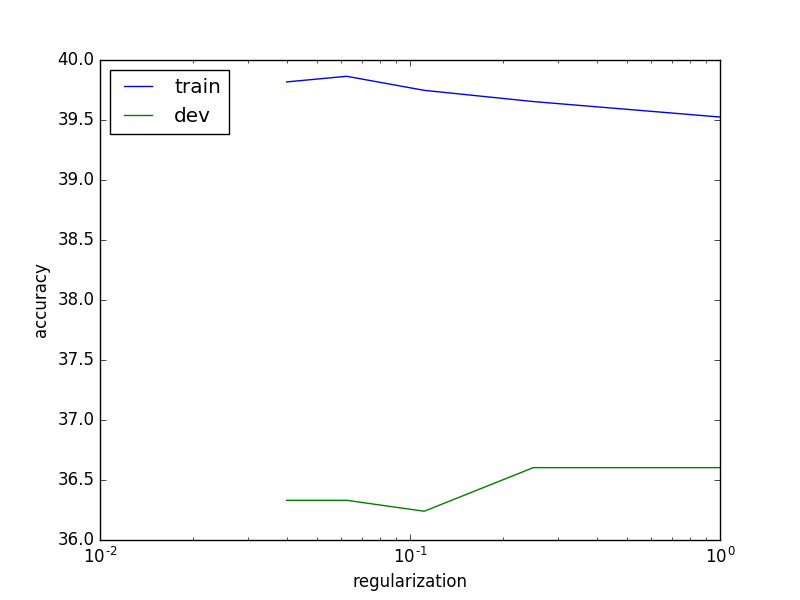
\includegraphics[scale=0.7]{q4_reg_v_acc.png}
\end{figure}

\noindent In Figure~\ref{figure:acc_vs_reg} we can see that as we increase the size of the regularization coefficient, the in-sample accuracy (the ``train'' line in blue) decreases. However, this same process increases the model's accuracy in the development set. This is what we expect to see: the larger penalty is decreasing the model's out-of-sample bias by reducing the degree to which the training data are being ``memorized''. 


\newpage


%----------------------
\subproblem{f}{Confusion Matrix (4 pts)}
\textit{We will now analyze errors that the model makes (with pretrained GloVe vectors). When you ran} \newline\verb|python q4_sentiment.py --pretrained|, \textit{two files should have been generated. Take a look at}\newline \verb|q4_dev_conf.png| \textit{\textbf{and include it in your homework writeup}. Interpret the confusion matrix in at most three sentences.} \\


\textbf{Answer:}\\

\begin{figure}[!htbp]\centering
	\label{figure:confusionmatrix}
	\caption{Confusion Matrix (Development Set)}
	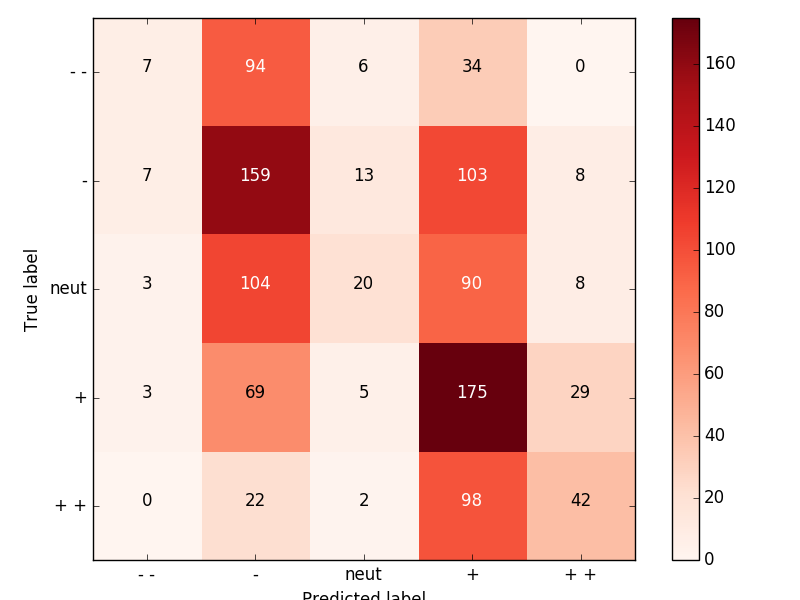
\includegraphics[scale=0.7]{q4_dev_conf.png}
\end{figure}

\noindent The confusion matrix shows us that the model has a difficult time predicting extremes on either end, even though they are fairly common in the training set. It also shows us that predicting the neutral category is difficult; the model tends to assign these cases to the ``negative'' class slightly more often than the ``positive'' class. Finally, while incorrect signs (in the binary sense) are present throughout, it is reassuring that in no instance did we assign a ``very positive(negative)'' sentence to the ``very negative(positive)'' class. \\

\noindent {\small PS. Apologies for the graphic being cut-off; it's not a {\LaTeX} problem, but is like that in the raw file as well.}


\newpage 

%----------------------
\subproblem{g}{Error Types \& Features (4 pts)}
\textit{Next, take a look at} \verb|q4_dev_pred.txt|. \textit{Choose 3 examples where your classifier made errors
and briefly explain the error and what features the classifier would need to classify the example correctly
(1 sentence per example). Try to pick examples with different reasons.} \\


\noindent \textbf{Answer:} \\

\begin{enumerate}
	\item ``\verb|and if you 're not nearly moved to tears by a couple of scenes ,| \newline \verb|you 've got ice water in your veins .|''
	\subitem $\bullet$ True $= +$; Predicted $= -$
	\subitem $\bullet$ In order to properly classify this sentence the model would need to have some feature about the idiom ``moved to tears'' being a positive phrase $w.r.t.$ film.
	%
	\item[] 
	%
	\item ``\verb|suffers from the lack of a compelling or comprehensible narrative .|''
	\subitem $\bullet$ True $= +$; Predicted $= --$
	\subitem $\bullet$ Here the issue is that ``compelling'' and ``comprehensible narrative'' are modified by the first word ``suffers''.
	%
	\item[]
	%
	\item ``\verb|it 's like watching a nightmare made flesh .|''
	\subitem $\bullet$ True $= --$; Predicted $= +$
	\subitem $\bullet$ This case is odd; a Google search brought up the full review in \textit{New York Magazine} by Peter Rainer (2002) in which the context suggests (to me) that the ``true'' label is incorrect. \footnote{\href{http://nymag.com/movies/articles/02/10/bloodysunday.htm}{You can see the full review by clicking here.}}
\end{enumerate}


\end{document}
